\documentclass[tikz,border=5pt]{standalone}
\usepackage[T1]{fontenc}
\usepackage{pgfplots}
\usepgfplotslibrary{groupplots}
\pgfplotsset{compat=1.18}
\definecolor{allowblue}{RGB}{0,88,138}
\definecolor{denyred}{RGB}{163,41,47}
\definecolor{certorange}{RGB}{166,95,0}
\begin{document}
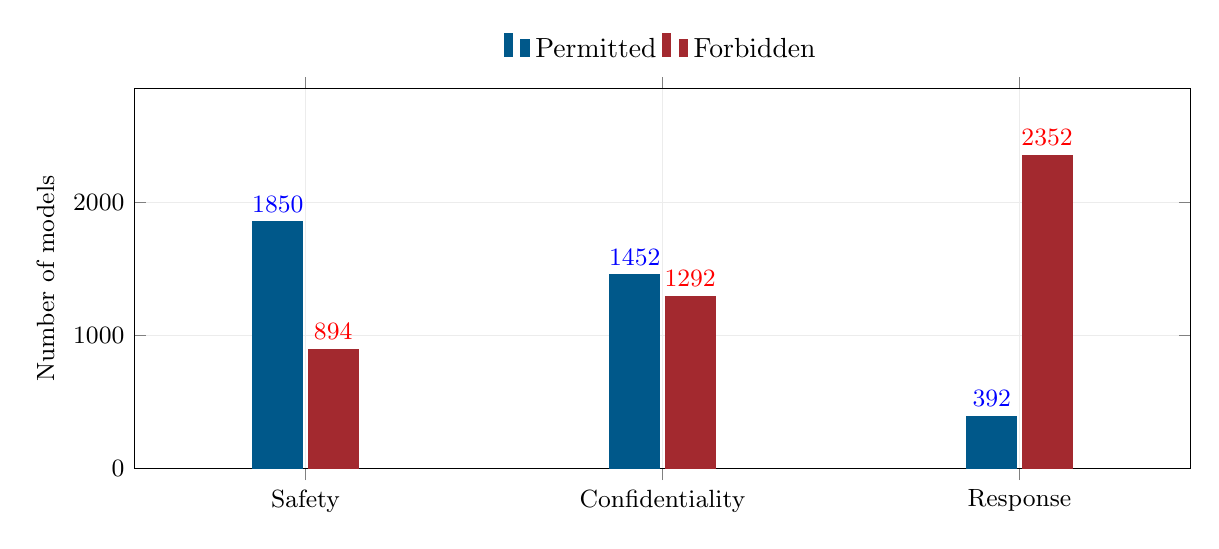
\begin{tikzpicture}
\pgfkeys{/pgf/number format/1000 sep={}}
\begin{axis}[width=15cm,height=6.4cm,ybar,bar width=18pt,
 symbolic x coords={Safety,Confidentiality,Response},xtick=data,
 enlarge x limits=0.24,ymin=0,ymax=2850,
 ylabel={Number of models},grid=major,grid style={gray!15},
 legend style={at={(0.5,1.04)},anchor=south,legend columns=2,draw=none},
 nodes near coords,every node near coord/.append style={font=\small},
 tick label style={font=\small},label style={font=\small}]
\addplot+[fill=allowblue,draw=allowblue] coordinates {(Safety,1850) (Confidentiality,1452) (Response,392)};
\addlegendentry{Permitted}
\addplot+[fill=denyred,draw=denyred] coordinates {(Safety,894) (Confidentiality,1292) (Response,2352)};
\addlegendentry{Forbidden}
\end{axis}
\end{tikzpicture}
\end{document}
